% !TEX root =  main.tex
\section{Introduction}

%Many AI tasks such as question answering require ability to interpret and reason about scenarios and situations.
Knowledge extraction and reasoning are central for many Artificial Intelligence systems. 
Recently introduced tasks such as {\em MCTest} reading comprehension challenge~\cite{richardson2013mctest}, grade-level science exams~\cite{clark2015elementary}, and process comprehension tasks~\cite{berantSrikumar14} serve as excellent benchmarks for developing reasoning-based question answering systems. 
These tasks test the ability of the systems to interpret and reason about scenarios and situations.
Knowledge requirements analysis for grade-level science exams shows the need for deep inference supporting knowledge~\cite{chb2013:akbc,clark2014:akbc}.
Also, even with advanced state-of-the-art reasoning techniques, shallow text-derived knowledge is ineffective due to lexical and syntactic variations in language~\cite{khot2015:emlnlp}.
Scalable acquisition of deeper semantic knowledge is essential for effective reasoning in these tasks. 

Much progress has been made on question answering involving simple facts~\cite{berant2013semantic,fader2014open,bordes2014open,reddy2014large}. 
This is in large part due to the availability of large scale curated relational knowledge bases such as Freebase, coupled with significant advances in automatic relation extraction~\cite{schmitz2012open,carlson2010toward,suchanek2007yago}. 
Similar advances in large scale inference-supporting knowledge is vital for making significant advances in reasoning-based QA tasks.

\eat{Recently introduced benchmarks such as {\em MCTest} reading comprehension challenge~\cite{richardson2013mctest}, grade-level science exams~\cite{clark2015elementary}, and process comprehension tasks~\cite{berantSrikumar14} motivate reasoning-based approaches to question answering (QA).
Our prior work on knowledge requirements analysis for the grade-level exams shows the need for deep inference supporting knowledge~\cite{chb2013:akbc,clark2014:akbc}.
Even with advanced state-of-the-art reasoning techniques, shallow text-derived knowledge is ineffective due to lexical and syntactic variations in language~\cite{khot2015:emlnlp}.
Recent work on process comprehension also shows that extracting richer semantic knowledge is more effective~\cite{berantSrikumar14}.
Scalable acquisition of deeper semantic knowledge is essential for effective reasoning in these tasks. }

In this work, we focus on knowledge acquisition methods with grade science exams as an end application. 
In particular we focus on a subset of knowledge about physical, chemical, and other natural phenomena.
The goal is to derive knowledge that allows effective reasoning about scenarios involving these phenomena. We refer to this as process knowledge. 
\footnote{Our representation and acquisition methods will be targeted towards the grade science benchmarks but the methodology is general and can be applied to other tasks and domains.}

\eat{Our vision is targeted acquisition of inference-supporting knowledge that can be used for reasoning tasks such as Question Answering (QA).
In particular we focus on knowledge acquisition for standardized test benchmarks such as grade-level science exams~\cite{clark2015elementary}.  Our prior work on these tasks provide strong motivation for reasoning based approaches~\cite{clark2014:akbc,chb2013:akbc}.
Lexical and syntactic variations render shallow text-derived knowledge ineffective for reasoning, even when using advanced state-of-the-art techniques~\cite{khot2015:emlnlp}. 
Deeper semantic representations are critical for effective reasoning.

This proposal investigates methods for acquiring knowledge about physical, chemical, and other natural phenomena.
The goal is to derive knowledge that allows effective reasoning about scenarios involving these phenomena. We refer to this as process knowledge. 
Our representation and acquisition methods will be targeted towards the grade science benchmarks but the methodology is general and can be applied to other tasks and domains.}

\subsection{Motivation}
%We illustrate the need for inference-supporting knowledge using two examples from 4$^{th}$ grade science exams. 
%These questions test the ability to recognize a process based on the description of a scenario. \\
We illustrate the need for inference supporting knowledge using the following example from a 4$^{th}$ grade science exam.
\begin{figure}[hbt]
	\begin{center}
	%12.08 x 2.9
	% 12.08 x 1.90
	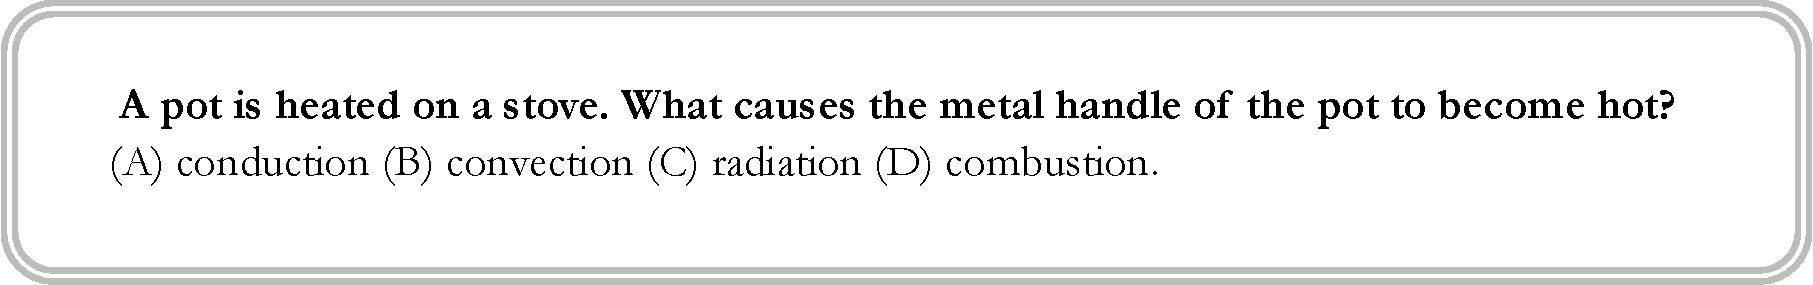
\includegraphics[width=6.04in,height=0.95in]{figures/single-question-stretch.pdf} 	
	\vspace{-1em}
	%\caption{\label{fig:questions} {Example Question from New York Regents Exam.}}
	\end{center}
\end{figure}

\eat{\begin{center}
\framebox{
\begin{minipage}{36em}
\begin{enumerate}
	\item {\em When plants use stored sugar for energy, they go through a process called\\
	(A) photosynthesis (B) transpiration (C) respiration (D) perspiration.}\\
	
	\item {\em A pot is heated on a stove. What causes the metal handle of the pot to become hot? \\
	(A) Conduction (B) Convection (C) Radiation (D) Combustion}. \\
\end{enumerate}

\end{minipage}

}
\\
\end{center}
}


%The knowledge necessary for this task is naturally expressed via simple semantic roles. 
\eat{The first question tests for knowledge about biological processes.
{\em Photosynthesis} and {\em respiration} both involve sugar and energy. 
Photosynthesis converts light energy to sugar, whereas (cellular) respiration releases energy in the sugar by breaking it down. 
Not surprisingly these processes are described using similar words, which makes bag-of-words style reasoning unreliable. 
Understanding the different roles that energy and sugar play in these processes, and knowledge of the main actions involved is key to effective reasoning.
}
%The second question requires reasoning about heat transfer mechanisms.
The question tests reasoning about heat transfer mechanisms.
To establish that conduction is the cause, a reasoning system must establish that there is some heat transfer happening through {\em direct contact}. 
We envision a system that first interpret the scenario and apply its knowledge about the heating process and the conduction process. 
In this case, the system needs to first identify {\em what is being heated} (the pot), and {\em what is the purported result} of the heating (the pot handle becoming hot). 
Then, knowledge about {\em heating} should allow it to conclude that the thing being heated (the pot) will become hot. 
Knowledge about {\em conduction} should suggest that anything {\em in direct contact} with a hot object (the pot handle) should also become hot.
Combining these bits the system can verify that the described scenario indeed matches the conduction process.
Replicating this type of reasoning requires the knowledge in a suitable computational representation.
%Specifically the knowledge about conduction should convey that there are two entities that are in direct contact, one of which is being heated or is hot, 
%and the result of conduction is that the other object also becomes {\em hot}. 

The knowledge required -- what is undergoing the process, what the result is and so on -- are naturally encoded as semantic roles.
PropBank and FrameNet are two of the highly successful efforts which provide this kind of semantic role based knowledge.
%for creating broad coverage semantic role based knowledge~\cite{}.
They have spurred tremendous advances in automatic semantic role labeling and their applications~\cite{}.
While these resources provide exhaustive coverage for modeling general open-domain actions,
they do not cover knowledge about scientific processes. 
FrameNet, for instance, does not have entries for nearly half of the processes described in 4th grade science exams. 
The coverage is likely worse for higher grade levels with deeper knowledge domains. 

\subsection{Proposal}

In response, we propose to build a knowledge base about physical, chemical, and biological processes from their textual descriptions. 

\subsubsection*{Representation}

Our primary motivation is to design a representation that facilitates reasoning while balancing extractability.
We propose to compose knowledge about each process using a set of pre-determined vocabulary of semantic roles and derive additional new roles automatically as needed.
While many competing role sets exist, we propose a role vocabulary that covers most inferential needs in the target process recognition dates~\cite{louvan2015:kcap}.
By leveraging a common vocabulary we expect to gain from shared learning for the same roles across different processes.

Similar to FrameNet we propose to determine roles with respect to the semantics of the process rather than with respect to the specific verb (or predicate) that is used to describe the process.
This canonicalization is desirable as it reduces reasoning time burden by eliminating need for steps that only establish equivalence of information realized via different predicates.

\begin{figure}[hb]
	\begin{center}
	%13.5 x 15.15
	%20.01 x 6.78
	%18.79 x 6.78
	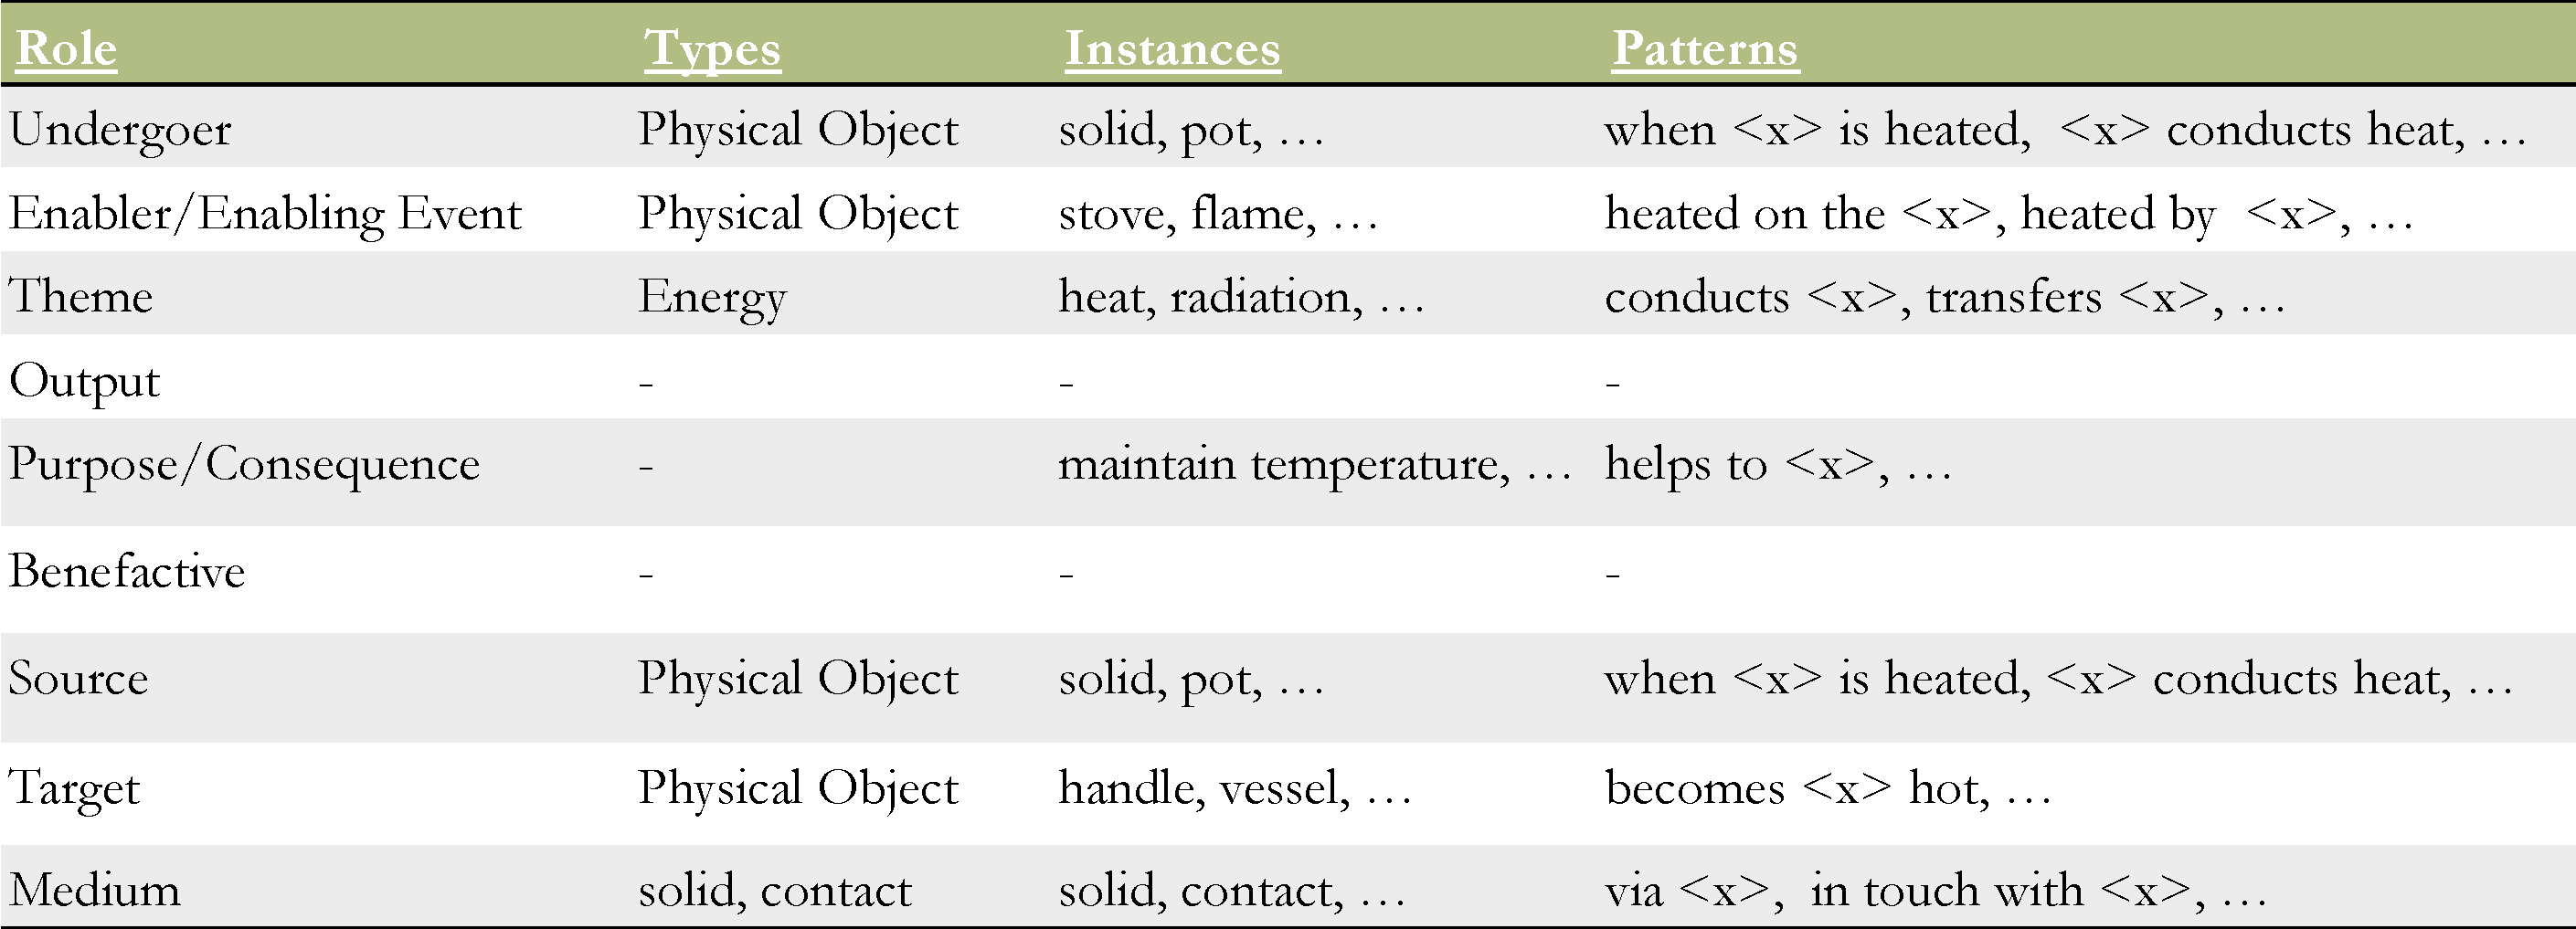
\includegraphics[width=6.26in,height=2.26in]{figures/processkb-snippet.pdf} 	
	\caption{\label{fig:kbsnippet} 
	{An example entry for the process {\em thermal conduction}.}
	}
	\end{center}
\end{figure}
With each role we include role fillers which are the frequent entries for that role, types which encodes class level information about the fillers, and syntactic argument realization patterns for these fillers.
We also include the source sentences from which the knowledge was derived.
Figure~\ref{fig:kbsnippet} shows an example for the envisioned knowledge. 
The table includes a set of pre-specified general purpose roles such as {\em Undergoer}, {\em Enabler} and also a process specific role {\em Medium} that is automatically derived from inspecting sentences that describe the process. 

%
\subsubsection*{Iterative Role Extraction and Joint Inference}

We devise an iterative procedure that exploits the abundance and variety of information on the web to acquire the necessary knowledge.

%The need for a canonicalized representation precludes the direct use of existing annotations or tools built for PropBank.
General semantic role labeling task is challenging because of the lexical and syntactic variations in role realizations. 
Handling the variations requires learning from large amounts of training data, which is laborious and requires expert labor.
Also as discussed earlier, existing semantic resources such as FrameNet or PropBank cannot be directly used for training as they do not cover the target concepts.
Rather than build a role labeler that can work on any sentence, we propose a simpler approach that works well on a smaller subset of sentences.

{\bf We tackle the role acquisition problem by explicitly searching for sentences that convey role information using specific patterns.}
%{\bf The main idea is a acquisition of knowledge from sentences that convey information in expected ways.}
Leveraging the vastness of the web greatly reduces the need to accurately identify roles in difficult to process sentences.
Using a set of manually constructed query patterns we find sentences which convey the roles using expected lexico-syntactic constructs. 
For instance "<process name> causes <x>" is a simple pattern that can be used to find the {\em result} role for a process. 
This strong expectation for how arguments are realized allows us to turn SRL into a simpler task of assessing the confidence on the extraction using features that generalize better across different processes.  
This allows us to substantially reduce the burden of annotating sentences for each process.
Even though PropBank and FrameNet data are not directly usable, the predicate-based roles and the frame structures can provide evidence for composing our target semantic roles. 
We propose to exploit these features to build a local sentence-level extractor.


Despite the targeted acquisition, local sentence-level extraction alone is not adequate, because not all lexico-syntactic patterns are unambiguous. 
For example, "evaporates into <x>" extracts steam, a {\em result}, as well as atmosphere, a {\em location}. 

{\bf A second key idea is to perform joint inference over multiple sentences to avoid errors in the local extraction}.
Because our goal is to acquire knowledge about a process, we turn the variety of expression on the web to our advantage. 
We build on prior work in Integer Linear Program (ILP) based semi-supervised and unsupervised induction approaches. 
The ILP attempts to find an assignment of roles that maximizes the sum of extraction confidences, 
while also minimizing disagreements in labels for similar text spans in similar sentences.

\subsubsection*{Assessment and Discovery}
While we start with a set of general purpose roles, {\em a priori} we don't assume which roles are applicable to each process as this manual assignment is not desirable from a scalability standpoint.
Also not all critical information may be covered by the set of roles that hand.

{\bf A third contribution of this proposal includes methods that identify the subset of roles that apply to a process and discover new roles not part of the general vocabulary}. 
As part of the targeted acquisition, we propose an iterative approach with methods to i) assess the coverage of the roles, ii) induce new roles by identifying consistently repeated arguments that don't fit existing roles, and iii) relevance feedback based query pattern generation to expand the knowledge.

\subsubsection*{Evaluation}

The generated knowledge base will be evaluated for intrinsic quality and external utility. For internal evaluations we will perform manual evaluation of the resulting KB. As part of the evaluation, {\bf we will also create a large scale curated KB, which relies on correcting the outputs from the system, rather than careful annotation of each sentence}. We will also generate a gold standard of the desired roles and role fillers for evaluating coverage. As an external evaluation we will use the knowledge base for answering process recognition questions. All the resources and evaluation test beds will be shared with the research community for further research.

\subsection{Prior Work and Contributions}

The motivation and direction for this proposal stems directly from our prior work on grade science exams.  Our earlier work studied knowledge requirements~\cite{chb2013:akbc}, developed inference-supporting rule knowledge bases~\cite{clark2014:akbc}, and investigated sophisticated state-of-the-art probabilistic reasoning methods for QA~\cite{khot2015:emlnlp}. Our ongoing preliminary work investigated the value of a handful of semantic roles in answering process recognition questions and identified the knowledge, representation, and reasoning gaps~\cite{louvan2015:kcap}. This proposal aims to address the central challenges that we've identified through these prior works.

Upon successful completion this project would have made the following contributions:
\begin{itemize}
\item Release of a knowledge base covering semantic representations of processes for grade level science.
\item Methods for gathering high quality sentences that cover a target set of roles. 
\item A joint inference method that reconciles roles across different sentences.  
\item Methods for assessing applicability, coverage and discovery of new roles.
\end{itemize}



